\chapter{相关算法及Hadoop分布式数据处理}
本文提出的推荐系统基于语义分析、%主成分分析、
协同过滤算法、Hadoop和MapReduce等几个基本算法及基本概念。
以下简单介绍这几个算法及概念。
\section{语义分析}
自然语言分析包含以下主要步骤:
\begin{enumerate}
	\item 句尾检测

	这一步主要是把一段文字分成一个有意义句子的集合\parencite{kiss2006unsupervised}。
	因为句子一般都含有思想的逻辑单元,所以句子的语法是可以预测的。
	而切词工作是建立在单个句子上的,所以分析文章一般从句尾检测开始。
	
	\item 切词
	
	这一步主要在单个句子上进行操作,将句子分为单个词。
	切词工作对于不同的文字有不同的切法,比如英文切词工作主要按空格切分,但还要注意不能混淆点号的意义;
	而中文没有空格,切词时要按照语料库是否存在该词来切分。

	\item 词义类型标记

	这一步主要是在切好的词语中标记词语的类型,比如是动词还是名词或者是长名词中的一部分。
	对于社交网络中的语言,比如推特或者微博,语言比较口语化,会出现大量动词名词混用情况\parencite{Gimpel2011Part,Owoputi2015Improved,Derczynski2013Twitter}。
	通过标记,机器甚至能指出名词或者是长名词是属于什么类型,比如是人,地点,或者组织。
	
	\item 分块
	
	这一步主要是在有逻辑意义的整句和复合标记的基础上分析词语。
	根据预先定义好的语法,将标记了类型的词语分成块。

	\item 提取主要内容

	这一步主要是进一步为分好的块标记名称或者类型,这与第三步词义类型标记不同,因为这一步以块为整体标记名称或者类型。
\end{enumerate}

其中每一步都很关键,因为一旦其中一步出错,误差会逐步传播,使得语义分析出严重错误。下面我们介绍计算自然语言分析准确度的方法。在语义分析完成后,统计以下数量:
\begin{center}
\begin{description}
	\item[TP]
	被正确识别为实体的词语
	\item[FP]
	本来不应该被正确识别为实体的但确实被正确识别为实体的词语
	\item[TN]
	本来不应该被正确识别为实体的,同时没有被正确识别为实体的词语
	\item[FN]
	本来应该被正确识别为实体的,但没有被正确识别为实体的词语
\end{description}
\end{center}
此时再定义精确度与召回率如下:
\begin{center}
\begin{description}
	\item[精确度]
	$precision= \frac{TP}{TP+FP} $
	\item[召回率]
	$recall= \frac{TP}{TP+FN} $
\end{description}
\end{center}
则可以用下式来描述语义分析模型的准确度为
\[
F= 2* \frac{precision*recall}{precision+recall}
\]
\section{协同过滤算法}
给定用户集合中有$M$个用户,物品集合中有$N$个物品。
用户对物品的评价为User-Item矩阵$R$,其中$R_{ij}$代表用户$i$对物品$j$的评分。
其中用$R_{ij}=?$表示用户$i$对物品$j$的评分未知。最基本的协同过滤算法所研究的问题为:基于$R$,给每位用户推荐一个不包含该用户已经评价过物品的列表,其中的物品按照符合用户兴趣程度递减排序。

有两种等效的协同过滤算法,一种是基于用户的协同过滤,另一种是基于物品的协同过滤。
基于用户的协同过滤算法通过对相似用户的评分求和来预测用户对目标物品的评分\parencite{resnick1994grouplens}。
其中可以用Pearson相关系数或者cos相似度来判断用户之间的相似程度\parencite{Singhal2001Modern}。
通常用距离最近的$K$个用户的评分求和来预测用户对目标物品的评分,如下面的公式,用户$i$对物品$j$的评分为:
\[
	\hat{R}_{ij} = \frac{1}{C} \sum_{k\in Z_i} sim(i,k)R_{kj}
\]
其中$Z_i$代表距离用户$i$最近的用户集合,$C$是放缩常数,$sim(i,k)$是用户$i$和用户$k$之间的相似度。
上式是基于用户协同过滤算法的最简形式\parencite{adomavicius2005toward},它能推广到其他复杂模型,比如引入细颗粒度的邻近权重因子\parencite{herlocker2000explaining},迭代寻找邻近方法\parencite{Zhang2007A},或者基于用户的个人资料计算用户相似度\parencite{shi2009exploiting}。

% \section{主成分分析}
% 在推荐系统中通常有超大的User-Item矩阵,即矩阵有超高维度,造成计算极其复杂。
% 许多维度是重合的,于是我们可以寻找一些隐藏的维度来表示这些重合的维度。
% 对于给定$m \times n$的秩为$k$的User-Item矩阵$X$,要找到$m \times k$的矩阵$U$和$k \times n$的$V$,满足
% \[
% X \equiv U \cdot V^\tau
% \]
% 其中矩阵$U$的每一行代表一个用户为$u_i$,矩阵$V$的每一行代表一个物品为$v_j$。目标是最小化
% \[
% argmin \sum_{i,j}(x_{i,j}-u_i\cdot v_j)^2
% \]
% 给定一个阈值$\epsilon$,通过以下步骤找到矩阵$U$和$V$:
% \begin{enumerate}
% 	\item 随机选择一个矩阵$V$;
% 	\item 固定矩阵$V$,优化矩阵$U$;对逐个用户$u_i$进行优化,即固定$v_j$,需要找到
% 	\[
% 	argmin_{u_i} \sum_{j\in P_i}(p_{i,j}-u_i\cdot v_j)^2
% 	\]
% 	这是线性最小二乘方程,可以得到
% 	\[
% 	u_i=(V_{*,i}^{\tau}V_{*,i})^{-1}V_{*,i}P_{*i}
% 	\]
% 	其中$V_{*,i}$是有来自用户$u_i$的评价的$V$的子集。
% 	\item 固定矩阵$U$,优化矩阵$V$,与上一步相似;
% 	\item 循环第2、3步,直到相关系数的变化量小于$\epsilon$,即可得到收敛解。
% \end{enumerate}
\section{Hadoop和MapReduce}
Google于03至06年公布了三篇论文,描述了GFS、BigTable、MapReduce三种技术以解决这些问题\parencite{Dean2004MapReduce,Ghemawat2003The,Chang2008Bigtable}。
由于Google并没有公布算法细节,因此由雅虎牵头,在06年左右建立了开源项目Hadoop,目的是根据Google的三篇论文,实现一个大规模的管理计算系统。

Hadoop的基础组件是Hadoop分布式文件系统(HDFS)。
HDFS的机制是将大量数据分布到计算机集群上,数据一次写入,但可以多次读取用于分析。
Hadoop的主要执行框架即MapReduce。
对于保存在分布式文件系统的数据,MapReduce在每个数据节点上进行本地运算。
\def\HDFSfront{
	\path (0,0) node(Splitn) [rectangle,draw] {Split(n)}
			(0,1) node {$\cdots$}
			(0,2) node(Split3) [rectangle,draw] {Split(3)}
			(0,3) node(Split2) [rectangle,draw] {Split(2)}
			(0,4) node(Split1) [rectangle,draw] {Split(1)}
			(0,5.5) node {\textbf{HDFS}};
	\draw (-1,-1) rectangle (1,6);
}
\def\HDFSend{
	\path (10,0) node(Partn) [rectangle,draw] {Part(n)}
			(10,1) node {$\cdots$}
			(10,2) node(Part3) [rectangle,draw] {Part(3)}
			(10,3) node(Part2) [rectangle,draw] {Part(2)}
			(10,4) node(Part1) [rectangle,draw] {Part(1)}
			(10,5.5) node {\textbf{HDFS}};
	\draw (9,-1) rectangle (11,6);
}
\def\mapper{
	\path (3.5,-1) node(Mapper4) [rectangle,draw] {\textbf{Mapper}}
			(3.5,0.5) node {$\cdots$}
			(3.5,2) node(Mapper3) [rectangle,draw] {\textbf{Mapper}}
			(3.5,3.5) node(Mapper2) [rectangle,draw] {\textbf{Mapper}}
			(3.5,5) node(Mapper1) [rectangle,draw] {\textbf{Mapper}};
}
\def\reducer{
	\path (7,1) node(Reducer2) [rectangle,draw] {\textbf{Reducer}}
			(7,2.5) node {$\cdots$}
			(7,4) node(Reducer1) [rectangle,draw] {\textbf{Reducer}};
}
\begin{center}
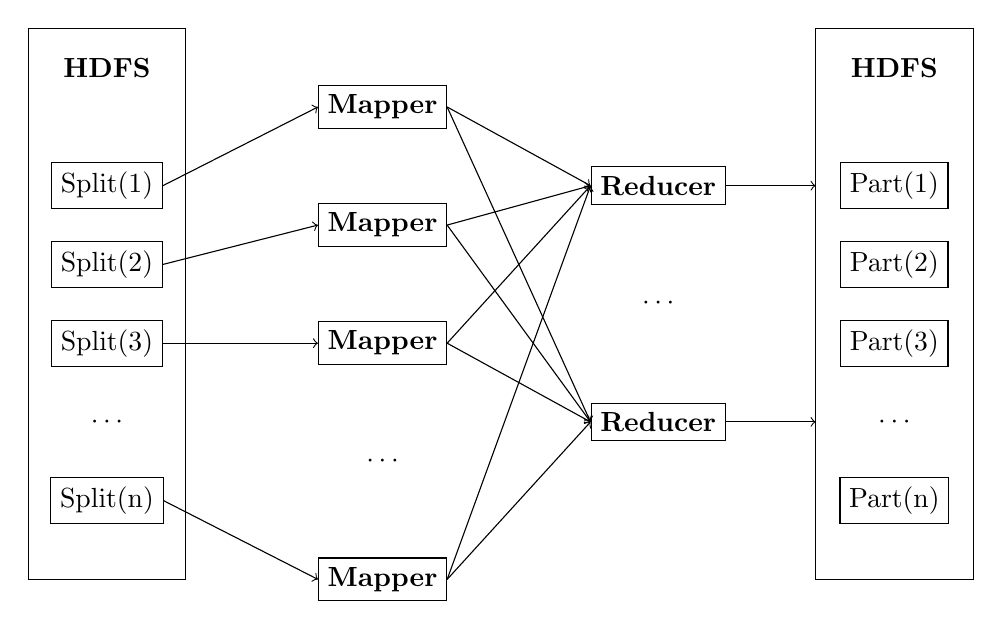
\begin{tikzpicture}
\HDFSfront
\mapper
\reducer
\HDFSend
\draw[->] (Split1.east) -- (Mapper1.west);
\draw[->] (Split2.east) -- (Mapper2.west);
\draw[->] (Split3.east) -- (Mapper3.west);
\draw[->] (Splitn.east) -- (Mapper4.west);
\draw[->] (Mapper4.east) -- (Reducer1.west);
\draw[->] (Mapper4.east) -- (Reducer2.west);
\draw[->] (Mapper3.east) -- (Reducer1.west);
\draw[->] (Mapper3.east) -- (Reducer2.west);
\draw[->] (Mapper2.east) -- (Reducer1.west);
\draw[->] (Mapper2.east) -- (Reducer2.west);
\draw[->] (Mapper1.east) -- (Reducer1.west);
\draw[->] (Mapper1.east) -- (Reducer2.west);
\draw[->] (Reducer1.east) -- (9,4);
\draw[->] (Reducer2.east) -- (9,1);
\end{tikzpicture}
\figurecaption{Hadoop的MapReduce工作流程图}
\end{center}
MapReduce框架包含两个阶段,map阶段和reduce阶段。
输入数据和计算后的输出数据都是一个(key,value)集合。
用$<k,v>$来表示这些键值对。
key主要用在reduce阶段,用来决定哪个value结合在一起。
用两个函数来表示这两个过程:
\begin{eqnarray}
\mathbf{Mapper} &:& <k1,v1> \rightarrow list<k2,v2> \\
\mathbf{Reduce} &:& <k2,list<v2>> \rightarrow list<k3,v3>
\end{eqnarray}
计算过程从map阶段开始,其中并行执行map函数同时把保存在分布式文件系统的输入数据切分。
进行每次切分就是指定一个map任务。
每个map函数的输出键值对基于中间生成的键进行哈希分区。
然后排序每个分区接着按照键的排序进行合并。
有同样的键的分区被分配到单独的reduce任务中,接着reduce函数输出最终结果。

在Hadoop的MapReduce工作流程中,一个工作记录服务器作为主节点把数据分成几部分作为map阶段的输入。
同时任务记录服务器作为数据节点保存map函数中间生成的结果到HDFS中。
Hadoop会基于地点计划分配MapReduce运算,同时提高集群整体的输入输出效率来减少运算的成本。
